%%%%%%%%%%%%%%%%%%%%%%%%%%%%%%%%%%%%%%%%%%%%%%%%%%%%%%%%%%%%%%%%%%%%%%%%%%%%%%%%
%2345678901234567890123456789012345678901234567890123456789012345678901234567890
%        1         2         3         4         5         6         7         8

\documentclass[letterpaper, 11 pt, conference]{ieeeconf}  % Comment this line out if you need a4paper
\usepackage{graphicx}
%\documentclass[a4paper, 10pt, conference]{ieeeconf}      % Use this line for a4 paper

\IEEEoverridecommandlockouts                              % This command is only needed if 
                                                          % you want to use the \thanks command

\overrideIEEEmargins                                      % Needed to meet printer requirements.

% See the \addtolength command later in the file to balance the column lengths
% on the last page of the document

% The following packages can be found on http:\\www.ctan.org
%\usepackage{graphics} % for pdf, bitmapped graphics files
%\usepackage{epsfig} % for postscript graphics files
%\usepackage{mathptmx} % assumes new font selection scheme installed
%\usepackage{times} % assumes new font selection scheme installed
%\usepackage{amsmath} % assumes amsmath package installed
%\usepackage{amssymb}  % assumes amsmath package installed

\title{\LARGE \bf
Data Mining Energy Usage
}


\author{Muci Yu$^{1}$ and Tim Robert-Fitzgerald$^{2}$% <-this % stops a space
\thanks{*This work was supported by Adam Eck, professor of Machine Learning at Oberlin College}% <-this % stops a space
\thanks{$^{1}$Muci Yu is with the Department of Economics and Environmental Studies, Oberlin College, Oberlin, OH 44074, USA
        {\tt\small myu2@oberlin.edu}}%
\thanks{$^{2}$Tim Robert-Fitzgerald with the Department of Computer Science, Oberlin College, Oberlin, OH 44074, USA
        {\tt\small trobertf@oberlin.edu}}%
}


\begin{document}



\maketitle
\thispagestyle{empty}
\pagestyle{empty}


%%%%%%%%%%%%%%%%%%%%%%%%%%%%%%%%%%%%%%%%%%%%%%%%%%%%%%%%%%%%%%%%%%%%%%%%%%%%%%%%
\section{INTRODUCTION}

Accurately forecasting energy demand is critical because it ensures grid operators can generate enough power to satisfy electricity consumption during peak demand and avoid building unnecessary power plant and transmission infrastructure. Because utility companies need to match peak demand but average demand is much less than peak, some equipment is left idle most of the time. By peak shaving, that is to say, reducing the peak consumption, utility companies save resources. To shave peaks, utility companies must be able to predict when the peaks will occur so they can distribute resources by scheduling when energy intensive activities will occur. Another more obvious but equally powerful use of predicting resource consumption is to give occupants feedback. Especially when predicted values deviate from actual readings, there could be fixable resource inefficiencies.

In this paper we will discuss approaches to predicting energy consumption. Specifically, we focus on a kind of neural network referred to as a LSTM (long short-term memory) which remembers information from previous instances. As the most important information when considering the current instance is the previous instance, LSTMs are apt for forecasting time series. Overall LSTMs were surprisingly effective, and our predictions match closely with the actual data.


\section{PROBLEM}

Researchers have employed many different machine learning techniques in approaching the building energy forecasting problem. Tso and Yau [1], for example, compared the performances of regression, decision tree and neural network in predicting building energy consumption. They used the square root of average squared error (RASE) as performance measurement and found that these three techniques yielded similar results, indicating the three methods were generally comparable in this problem. However, they did point out the advantage of decision tree over other two methods, that is, it could produce a model which may represent interpretable rules or logic statements. Tsanas and Xifara [2] also compared the performance of decision tree versus regression, but they used their extended models, random forest (RF) and iteratively reweighted least square (IRLS), respectively. They showed that regression may fail to account for multicollinearity, but the decision tree mechanism can optimize the selection of the variable for each split and thus internally account for redundant and interacting variables. Their results indicated that RF algorithm was better than the IRLS, as the former generated much smaller errors than the later.

Rather than using one of the machine learning algorithms discussed above, we employ neural networks to predict resource consumption. Unlike decision trees, the model neural networks build can be manipulated by changing the edge weights. This feature is pivotal for us as we want to be able to introduce new data to the model without having to rebuild it from scratch. Furthermore, the model we build does not need to be human-interpretable. Rather, it is more important that we are able to model the often erratic, non-linear behaviour of building consumption. We focus on LSTMs because they are especially good at sequential learning. Unlike vanilla neural networks, the neurons in LSTMs have loops so that they may remember certain characteristics of the previous instances. By connecting previous information to the present instance LSTMs can learn sequences where instances are characterized by where in time they are placed.

The data set we use contains a wide variety of buildings from residential houses to large office buildings, all of which are located in Oberlin, OH. In total, data were collected for 822 meters across 96 buildings. These buildings included residence halls (33 total), residential houses (15 total), offices (4 total), dining facilities (12 total), academic buildings (18 total), government buildings (6 total), municipal buildings (1 total), laboratories (1 total), industrial buildings (1 total), administrative buildings (1 total), libraries (1 total), exhibit halls (1 total), and elementary schools (1 total). We collected 4 years of data for every meter at day resolution, that is to say, one data point per day, and 2 years of data at hour resolution. Overall, we trained our models on over 26 million data points totaling more than a gigabyte of storage.

This data was downloaded to a MySQL database using the BuildingOS API. To replicate our project with a different data set, create a PHP script called db.php in the bos directory which should create a new PDO object called \texttt{\$db}. Then replace the \texttt{CLIENT\_ID}, \texttt{CLIENT\_SECRET}, \texttt{USERNAME}, \texttt{PASSWORD} constants in class.bos.php with the appropriate values which can be obtained while setting up an API account in the BuildingOS interface. Run the \texttt{getOrganizations()} method as done in meta\_data.php to enumerate the organizations your BuildingOS account has access to, and run \texttt{syncBuildings()} on the desired organizations as demonstrated in meta\_data.php. Once the database is populated with a list of buildings, data can be downloaded by running meter\_data.php. By default, meter\_data.php is set to download hour resolution data in week chunks.

\section{SOLUTION}

Our LSTM implementation used Keras in conjunction with TensorFlow. Keras is a high-level API meant to work with TensorFlow that greatly simplifies the creation of neural networks. Our network contains two LSTM layers. The first layer is sized proportionally to the shape of the input data. The second LSTM layer has a fixed but configurable number of neurons optionally set by providing a command line argument. We use a linear activation function and the state-of-the-art Adam optimizer algorithm as these produced the most accurate results. To address overfitting, we set the dropout rate to 20\%. According to researchers at the University of Toronto, “the key idea is to randomly drop units (along with their connections) from the neural network during training" which “prevents units from co-adapting too much” [4]. 


\section{EXPERIMENTAL SETUP}

Our project consists of three primary python files, buildingNN.py, predictor.py, and retrain.py. These files require python packages which can be installed through pip, python’s package manager. Specifically, the required packages are pymysql, tensorflow, numpy, matplotlib, keras, h5py, sklearn, and pandas. Once these packages are installed, buildingNN.py can be run to generate models. BuildingNN.py takes up to 7 command line arguments, all of which are optional. In the order they are expected, the arguments are for data resolution (day or hour, defaults to hour), whether or not to chart the results (chart or nochart, defaults to nochart), a specific meter ID to train on (if not given a model will be created for all meters), number of epochs to train for (defaults to 5), the training percentage (defaults to 90\%), the number of neurons (defaults to 100), and the learning rate (defaults to 0.001). For example, running \texttt{python3 buildingNN.py hour chart 266 5 0.9 100 0.1} would build a network for meter 266 using hour resolution data, 5 epochs, 90\% training percentage, 100 neurons, 0.1 learning rate and would chart the results while running \texttt{python3 buildingNN.py day nochart} would generate a network for all the meters in the database using day resolution data without drawing a chart for each meter. Once models are in the database, predictions can be made by running \texttt{python3 predictor.py [meter\_id] [resolution]}. If a model needs to be retrained, run \texttt{python3 retrain.py [meter\_id] [resolution]}.

\subsection{Training}

We represented our instances as windows of data points with each window trying to predict the value following the last data point in the window. The number of data points in the windows is determined by our window\_size parameter. We made the windows by iterating over the data points one by one. For example, if our data set was  $<t_0, t_1, t_2, t_3, \ldots t_n>$ and the window size was 7, then our instances would be $<t_0, t_1 \ldots t_6>$, $<t_1, t_2 \ldots t_7>$, ... $<t_{n-7}, t_{n-6} \ldots t_{n-1}>$ and their labels would be $<t_7, t_8, t_9, \ldots t_n>$. 

We did not split the data points into training set and testing set randomly, because it is likely that the energy consumption at time t influences next period t+1. Randomly selecting data would eliminate the strictly sequential nature of our data. Instead, after choosing a training percentage, we selected the oldest percentage portion of data points as our training data and the rest as testing data. Within the training set, a validation set, if any, was selected with similar method. 

\subsection{Evaluation}

We evaluated model accuracy by calculating the mean squared error (MSE) and normalized root-mean-square deviation (NRMSD) of our predictions as well as visually comparing charts of predictions overlayed on the actual data. The MSE and NRMSD are defined as,

$$
NRMSD = \frac{RMSD}{y_{max} - y_{min}}
$$
and
$$
MSE = \frac{1}{n} \sum_{i=1}^{n} (Y_i - \hat{Y_i})^2
$$

where RMSD is the square root of MSE. 

The MSE is useful to investigate how the model’s performance changes by modifying certain parameters. However, the MSE is dependent on the scale of data, which suggests that the MSE is not meaningful if we are comparing data sets with different scales. Since we will explore different normalization methods, the scale of data will change. In this case, we use NRMSD to compare how different normalization methods affect the performance. When running the model, we receive reports on the MSE of training and validation sets at every epoch as well as a final MSE and NRMSD report for the testing set at the end. 


\subsection{Tested parameters}

We tried a variety of configurations and instance representations to building our model. First, we tried representing a single data point as an instance. This worked poorly, however, and we instead partitioned the data into contiguous windows which each represent an instance. The size of the window depends on the resolution of the data. For example, the window size for hour resolution data is 24 while the window size for day resolution data is 7. This forces the network to learn the characteristics of a period of time — a day in the case of hour resolution and a week in the case of day resolution, capturing humans’ behavioral cycles — rather than an arbitrary point. Second, we tried training on all data for similar meters, that is to say, meters of the same resource type. Doing so gave inaccurate results as the nuances of a particular meter are lost; even meters of the same resource type can have very different usage patterns. Third, we tried normalizing the data in different ways. Normalization had the largest effect on performance as without normalization the results were comparable to random guesses. Fourth, we tried adjusting the number of neurons. As illustrated in chart figure 2, accuracy increases as the number of neurons rise, but only until a certain point. At 1000 neurons performance is optimal. Additional neurons cause less accuracy, presumably because of overfitting. Fifth, we tried adjusting the learning rate, which produces odd results which we discuss in detail later. Finally, we tried adjusting the number of epochs the training happens for. Unsurprisingly, training for longer amounts of time increased accuracy, but with diminishing marginal returns.

\vspace{5pt}

\begin{figure}[h]
\caption{}
\centering
\includegraphics[scale=.3]{standardscaler_convertrange.png}
\end{figure}

\begin{figure}[h]
\caption{}
\centering
\includegraphics[scale=.3]{nn.png}
\end{figure}

\begin{figure}[h]
\caption{}
\centering
\includegraphics[scale=.3]{lr.png}
\end{figure}

\section{RESULTS}

Overall our project illustrates how powerful of a tool neural networks can be. Our network was given no information other than the raw meter readings and the sequence they were recorded in, but the network nonetheless accurately predicted future consumption. Because we gave the network no metadata about the meters, it is likely the model suffered from omitted-variable bias. Still, the network made accurate predictions suggesting neural network are good at compensating for the missing factor my over- or underestimating the influence of other variables. Indeed, neural networks find relationships in data too complex for humans to parse out.

Figure 4 and Figure 5 show our prediction results. In both cases, the results are fairly accurate, as their MSEs are just around 0.2. Also, graphically, our predicted results (shown as colored lines) fit with the actual values (shown as the blue line) well.

\begin{figure}[h]
\caption{}
\centering
\includegraphics[scale=.3]{id266_hour_epochs20_ws24_nn100_StandardScaler.png}
\end{figure}

\begin{figure}[h]
\caption{}
\centering
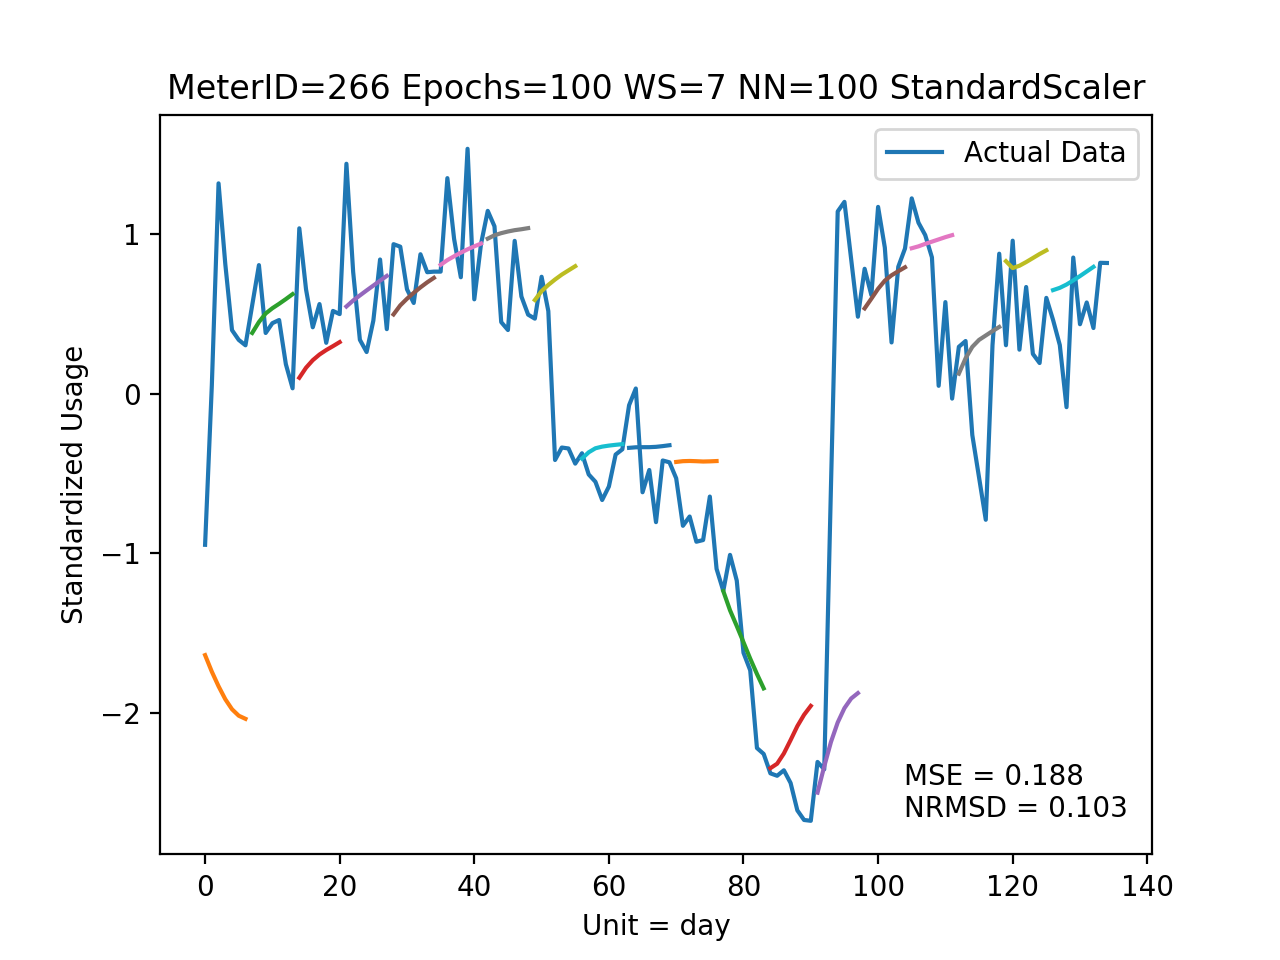
\includegraphics[scale=.5]{id266_day_epochs100_ws7_nn100_StandardScaler.png}
\end{figure}

Our experimental setup reveals how influential tuning the hyper parameters can be. Indeed, these configuration variables are powerful ways to change the fundamental architecture of the network with a line of code. Exploring different combinations of neurons, learning rates, epochs, and normalization of the instances led to major changes in prediction. 

Learning rates in particular had an interesting effect on performance. As chart figure 3 shows, a higher learning rate generally leads to less accuracy. This is to be expected, however, at various points increasing the learning rate actually increased accuracy, as represented by the dip in the MSE when increasing the learning rate from 0.4 to 0.5. Furthermore, a very high learning rate caused results to be unstable; the same network configuration would produce different results on the same data. We theorize this happens because a high learning rate causes the gradient descent to get stuck in local minima which are different depending on the learning rate.

As mentioned, normalization had the largest effect on performance as before we implemented normalization (commit hash: 7051ab58fd5f92adda9f5d8afedf7f43ab50e942) results were garbage. After normalization, however (commit hash: 0a4f78a76f2441aad9f0359c6347ca6a0d8cfc5f), results immediately improved. Indeed, the power of normalization can not be understated. Without normalization, the network is learning the scales of the numbers rather than the patterns of resource usage. Our first attempt at normalization used scikit-learn’s StandardScaler which transforms the data so that the standard deviation is 1 and the mean is 0. We also tried writing our own method, convertRange, which simple scales every number in our data set to a 0-1 range. As one can see in figure 1, both approaches worked decently well although StandardScaler was marginally more accurate.




\section{CONCLUSION AND FUTURE WORK}

While there are many approaches to forecasting time series, neural networks are the most flexible and accurate. Their ability to update their model without restarting from scratch is indispensable. Furthermore, neural networks make use of large data sets whereas with decision trees only having the minimal amount of data necessary to describe the problem is necessary. LSTMs are especially well suited for time series forecasting as they can relate previous instances to the current instance.

A potential extension of this project could be to implement fault detection which involves finding anomalous data that could be caused by faulty construction, malfunctioning equipment or inappropriate operating procedures. Another possible extension would be to include more information such as building occupancy. We attempted to use Oprestissimo to obtain occupancy information for academic buildings based on class schedule but we were never able to obtain access to this data set.


\addtolength{\textheight}{-12cm}   % This command serves to balance the column lengths
                                  % on the last page of the document manually. It shortens
                                  % the textheight of the last page by a suitable amount.
                                  % This command does not take effect until the next page
                                  % so it should come on the page before the last. Make
                                  % sure that you do not shorten the textheight too much.

%%%%%%%%%%%%%%%%%%%%%%%%%%%%%%%%%%%%%%%%%%%%%%%%%%%%%%%%%%%%%%%%%%%%%%%%%%%%%%%%




\begin{thebibliography}{99}

\bibitem{c1} G. K.F. Tso, K. K.W. Yau, Predicting electricity energy consumption: A comparison of regression analysis, decision tree and neural networks, In Energy, Volume 32, Issue 9, 2007, pp. 1761-1768
\bibitem{c2} A. Tsanas, A. Xifara, Accurate quantitative estimation of energy performance of residential buildings using statistical machine learning tools, In Energy and Buildings, Volume 49, 2012, pp. 560-567.
\bibitem{c3} I. Khan, A. Capozzoli, S. P. Corgnati, T. Cerquitelli, Fault Detection Analysis of Building Energy Consumption Using Data Mining Techniques, In Energy Procedia, Volume 42, 2013, pp. 557-566.
\bibitem{c4} Srivastava, N., Hinton, G., Krizhevsky, A., Sutskever, I., & Salakhutdinov, R. (2014). Dropout: A Simple Way to Prevent Neural Networks from Overfitting [Abstract]. Journal of Machine Learning Research, 15. Retrieved from http://www.cs.toronto.edu/~rsalakhu/papers/srivastava14a.pdf






\end{thebibliography}




\end{document}
